\clearpage
%%=========================================
\section[Surface Analysis of Substrate C with Surface Pre-Growth Preparation]{Surface Analysis of Substrate C with Surface Pre-Growth Preparation%
    \sectionmark{Surface Analysis of Pre-Growth Substrate C}}\sectionmark{Surface Analysis of Pre-Growth Substrate C}\label{sec:subCb}

The ultimate goal for the \ac{mbe} preparation etch is to provide a clean, smooth, and well-ordered surface to minimise growth defects.

%%=========================================
\subsection{Particles}

\begin{figure}
    \centering
    \begin{subfigure}[t]{\textwidth}
          \begin{minipage}[t]{0.49\linewidth}
            \centering
            
\includegraphics[width=\linewidth]{unknown.png}
          \end{minipage}
          \hspace{0.02\linewidth}
          \begin{minipage}[t]{0.49\linewidth}
            \centering
            
\includegraphics[width=\linewidth]{unknown.png}
          \end{minipage}
        \caption{\todo{Add caption}}\label{fig:add_label}
    \end{subfigure}
    \par\bigskip
    \begin{subfigure}[t]{\textwidth}
          \begin{minipage}[t]{0.49\linewidth}
            \centering
            
\includegraphics[width=\linewidth]{unknown.png}
          \end{minipage}
          \hspace{0.02\linewidth}
          \begin{minipage}[t]{0.49\linewidth}
            \centering
            
\includegraphics[width=\linewidth]{unknown.png}
          \end{minipage}
        \caption{\todo{Add caption}}\label{fig:add_label}
    \end{subfigure}
    \par\bigskip
    \begin{subfigure}[t]{\textwidth}
          \begin{minipage}[t]{0.49\linewidth}
            \centering
            
\includegraphics[width=\linewidth]{unknown.png}
          \end{minipage}
          \hspace{0.02\linewidth}
          \begin{minipage}[t]{0.49\linewidth}
            \centering
            
\includegraphics[width=\linewidth]{unknown.png}
          \end{minipage}
        \caption{\todo{Add caption}}\label{fig:add_label}
    \end{subfigure}
    \caption[\Ac{sem} images and \ac{eds} spectra of particles found on substrate C after surface pre-growth preparation.]{High resolution \acf{sem} images of particles found on substrate C after surface pre-growth preparation and the corresponding \acf{eds} spectra of the particles.}\label{fig:subCb_sem_w_eds}
\end{figure}

\begin{figure}[htbp]
\ContinuedFloat
    \centering
    \begin{subfigure}[t]{\textwidth}
          \begin{minipage}[t]{0.49\linewidth}
            \centering
            
\includegraphics[width=\linewidth]{unknown.png}
          \end{minipage}
          \hspace{0.02\linewidth}
          \begin{minipage}[t]{0.49\linewidth}
            \centering
            
\includegraphics[width=\linewidth]{unknown.png}
          \end{minipage}
        \caption{\todo{Add caption}}\label{fig:add_label}
    \end{subfigure}
    \captionsetup{list=no}
    \caption{\emph{(continued)}}
\end{figure}

%%=========================================
%\section{AFM Study of Etched Substrate C}
\subsection{Surface Roughness}
\begin{figure}[htbp]
    \centering
    \begin{subfigure}[t]{\linewidth}
    \centering
        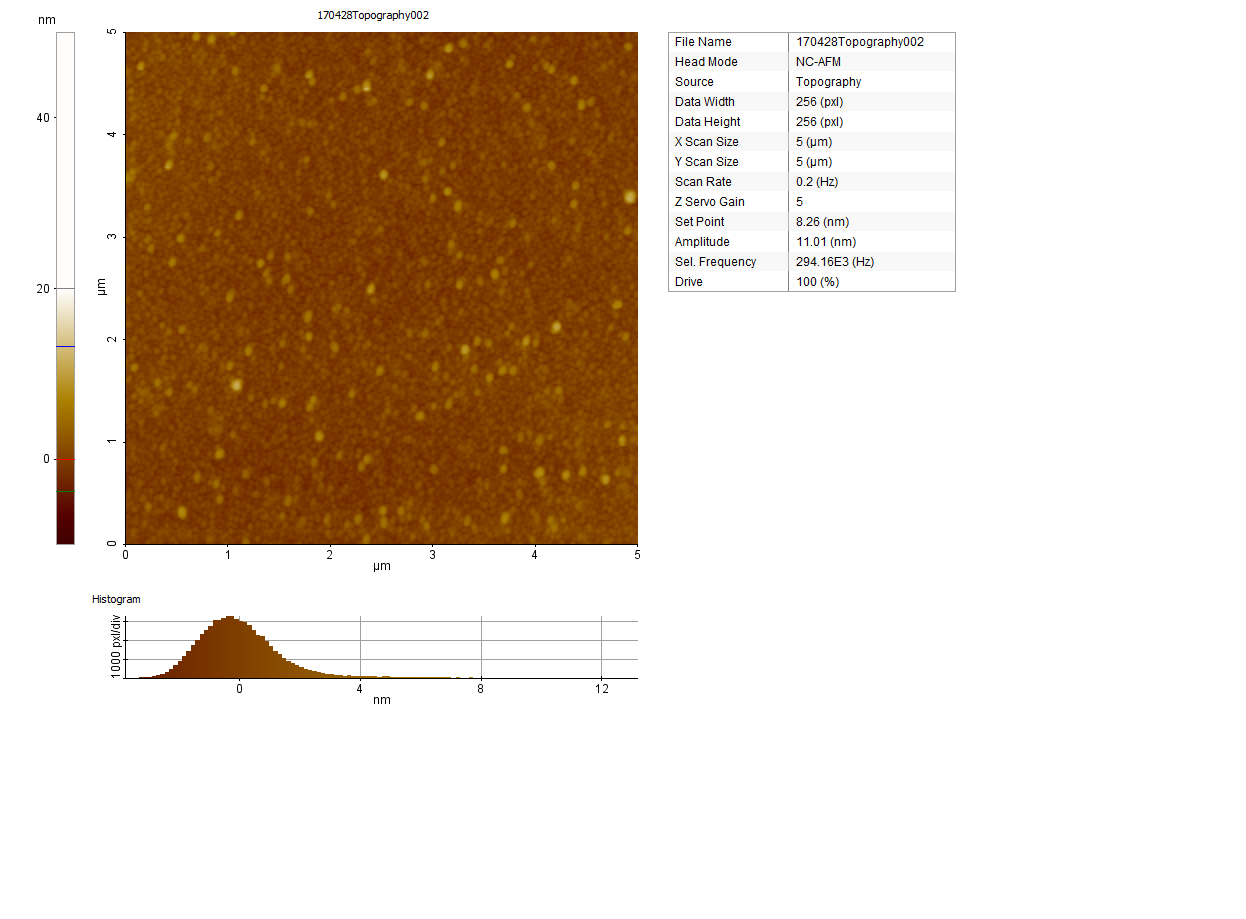
\includegraphics[width=0.5\linewidth,trim={0cm 12cm 21cm 0cm},clip]{170428Topography002_centre.png}
        \caption{Near centre, \ac{rms} roughness \SI{1.4}{\nano\metre}.}  %\SI{0.85}{\nano\metre}}
    \end{subfigure}%
    \par\bigskip
    \begin{subfigure}[t]{\linewidth}
    \centering
        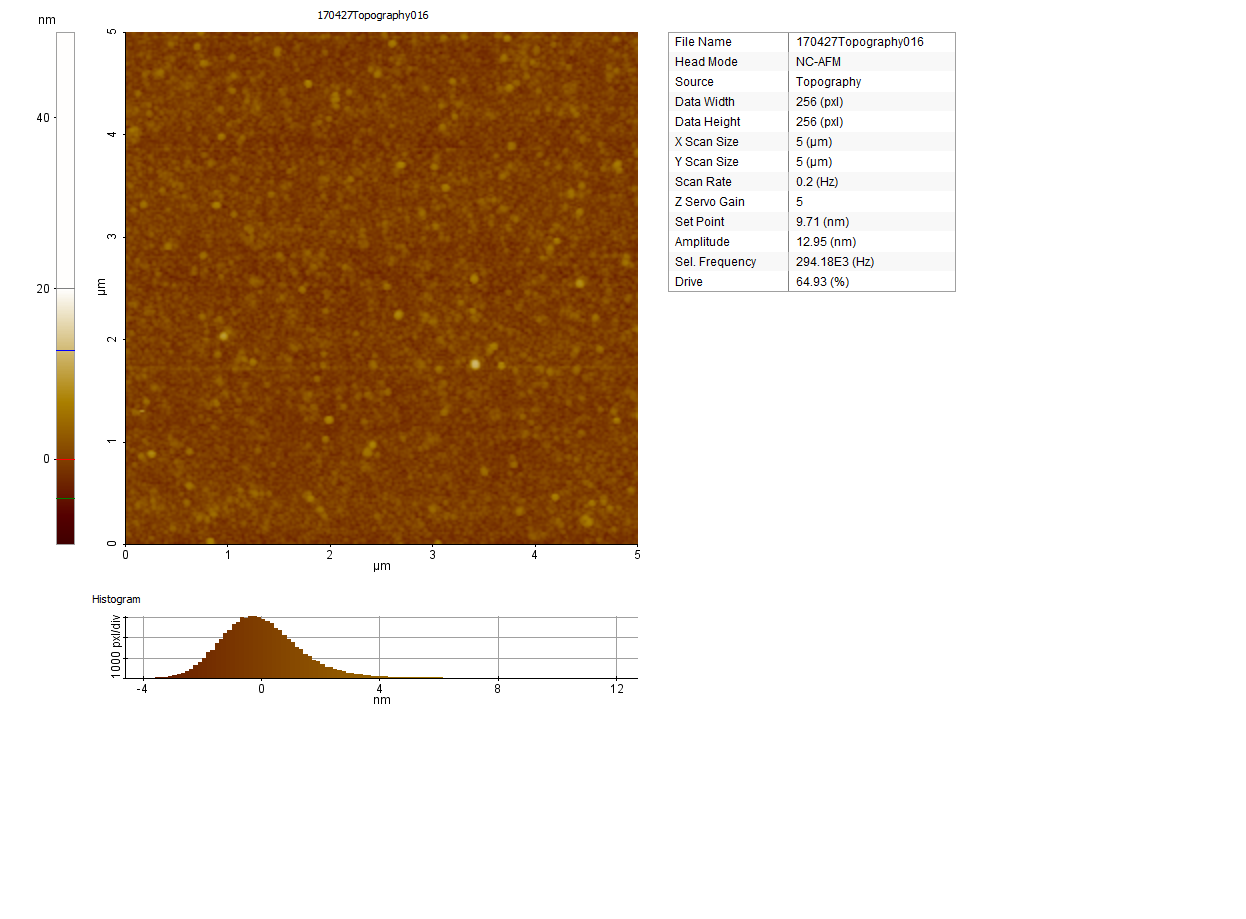
\includegraphics[width=0.5\linewidth,trim={0cm 12cm 21cm 0cm},clip]{170427Topography016_upperedge.png}
        \caption{Near upper edge, \ac{rms} roughness \SI{1.4}{\nano\metre}.}  %\SI{0.77}{\nano\metre}}
    \end{subfigure}%
    \par\bigskip
    \begin{subfigure}[t]{\linewidth}
    \centering
        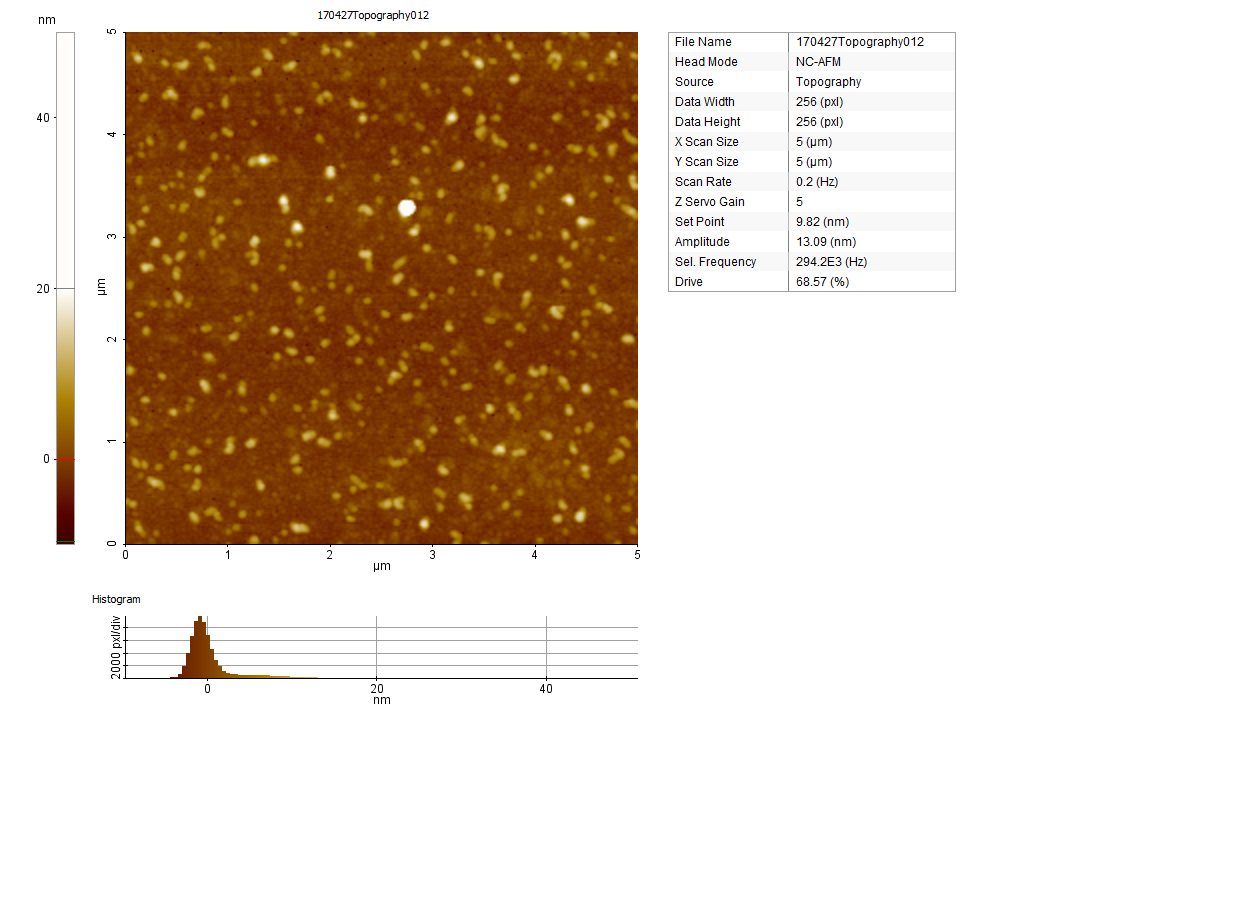
\includegraphics[width=0.5\linewidth,trim={0cm 12cm 21cm 0cm},clip]{170427Topography012_upperleftcorner.png}
        \caption{Near upper left corner, \ac{rms} roughness \SI{2.8}{\nano\metre}.}  %\SI{1,04}{\nano\metre}}
    \end{subfigure}%
    \caption[\Ac{afm} of substrate C with surface pre-growth preparation.]{\Acf{afm} measurements of substrate C with surface pre-growth preparation. Images of a $\SI{5}{\micro\metre}\times\SI{5}{\micro\metre}$ area are taken at the centre, edge, and corner of the substrate.}
    \label{fig:afm_subCb}
\end{figure} % AFM, substrate C, with surface pre-growth preparation.

%%=========================================
\subsection{Impurity Analysis}
\begin{table}[htbp]
    \centering
    \caption[\Ac{eds} impurity analysis of substrate C with surface pre-growth preparation.]{Results of the \acf{eds} impurity analysis at three different locations on the $15\times15$ \SI{}{\milli\metre^2} (211)B \ac{czt} substrate C with surface pre-growth preparation (atomic concentration \%). The X-ray signal is acquired from a $\SI{1270}{}\times\SI{890}{\micro\metre^2}$ area centred around the given $X$ and $Y$ values at a magnification of 100$\times$.}\label{tab:subCb_eds_analysis}
    \begin{tabu} to 1.0\textwidth { X[1,c] X[1,c] X[1.125,c] X[1.125,c] X[1.125,c] X[1.125,c] X[1.125,c] X[1.125,c] X[1.125,c] }
    \hline
        \textbf{$X$} (\SI{}{\milli\metre}) &  \textbf{$Y$} (\SI{}{\milli\metre}) & \textbf{\ce{Te}} (at.\%) & \textbf{\ce{Cd}} (at.\%) & \textbf{\ce{Zn}} (at.\%) & \textbf{\ce{Al} } (at.\%) & \textbf{\ce{Si}} (at.\%) & \textbf{\ce{C}} (at.\%) & \textbf{\ce{O}} (at.\%) \\
        \hline
         \SI{1.0}{} & \SI{14.0}{} & \SI{45.16}{} & \SI{45.26}{} & \SI{1.40}{} & \SI{1.79}{} & \SI{0.54}{} & \SI{5.85}{} & \SI{0}{} \\
         \SI{7.5}{} & \SI{14.0}{} & \SI{44.91}{} & \SI{44.93}{} & \SI{1.43}{} & \SI{2.33}{} & \SI{0.53}{} & \SI{5.86}{} & \SI{0}{} \\
         \SI{7.5}{} & \SI{7.5}{}  & \SI{45.02}{} & \SI{44.88}{} & \SI{1.45}{} & \SI{2.14}{} & \SI{0.52}{} & \SI{6.00}{} & \SI{0}{} \\
         \hline
    \end{tabu}
\end{table}

%%=========================================